%!TEX root = ../../common/main.tex

\section{Data preparation}
\label{sec:measurement_of_sin2beta:data_preparation}

The presented analysis is performed on a dataset collected by the \LHCb
experiment during two run periods in 2011 and 2012, dubbed
\enquote{\RunOne}\footnote{In contrast to the second \enquote{\RunTwo} period
scheduled to start in 2015 and last until mid 2018.}.

The 2011 subsample has an integrated luminosity of
$\SI[separate-uncertainty=true]{1.00\pm0.04}{\per\femto\barn}$ at a
centre-of-mass energy of $\sqrt{s}=\SI{7}{\TeV}$, while the 2012 subsample has
an integrated luminosity of
$\SI[separate-uncertainty=true]{1.990\pm0.024}{\per\femto\barn}$ at
$\sqrt{s}=\SI{8}{\TeV}$.

The $\BdToJpsiKS$ decay candidates are reconstructed in the $\JpsiToMuMu$ and
$\KSToPiPi$ final state. In order to enhance the purity of the signal
candidates, several selection steps are performed. At first a two-layer
\emph{trigger} system selects events from the \protonproton collisions (\cf
\cref{sec:measurement_of_sin2beta:data_preparation:trigger}). Then a loose and very general
selection, the so called \emph{stripping} is applied to the triggered data
written to tape (\cf
\cref{sec:measurement_of_sin2beta:data_preparation:stripping}). The final step
is an offline selection of the remaining candidates that is further adjusted to
the specific decay and the reconstructed final state (\cf
\cref{sec:measurement_of_sin2beta:data_preparation:offline_selection}).

Besides reducing the background level and enhancing the fraction of signal in
the data set, the selection tries to minimise a possible bias of the measured
\Bd lifetime caused by selection steps that preferably remove candidates with
small decay times. If it is inevitable, then at least the biasing effects should
be understood and accounted for (\cf
\cref{sec:measurement_of_sin2beta:resolution_and_acceptance:acceptance}).

\subsubsection*{Global decay chain fit}
In order to correctly comprise correlations and uncertainties on vertex
positions, particle momenta, flight distances, decay times, and invariant
masses, a global decay chain fit (\acs{DTF}) \cite{Hulsbergen:2005pu} is
performed. Instead of fitting \enquote{leaf-by-leaf} starting from the final
state particles to determine the parameters of their composite mother particle,
then repeating this step until the initial \bhadron is reached, the \DTF fit
extracts all parameters in the decay chain simultaneously.

Entities decorated with the expression \dtfpv stem from a \DTF fit where the
knowledge about the \PV has been used to constrain the production
vertex of the \Bd meson, while the expression \dtf means that additionally to
the \PV constraint the \jpsi and \KS invariant masses are constrained to their
masses listed by the \PDG ($m_{\KS}^{\text{\acs{PDG}}}=\SI{497.614}{\MeVcc}$,
$m_{\jpsi}^{\text{\acs{PDG}}} = \SI[per-mode=symbol]{3096.916}{\MeVcc}$, see
\cite{Agashe:2014kda}) inside the \DTF fit. In the stripping and if not stated
otherwise the much simpler leaf-by-leaf fitting was used.

\subsubsection*{Observables}

Throughout the analysis, several observables are used: the \Bd invariant mass
$\obsMass$, the decay time of the \Bd in its rest frame $\obsTime$, the \Bd
decay time error estimate $\obsTimeError$, and the tag decisions
\obsTagOSSS and mistag estimates \obsEtaOSSS of the opposite site and same side
tagging algorithms (\cf \cref{ch:flavour_tagging}).
\Cref{tab:measurement_of_sin2beta:data_preparation:observables} summarises all
used observables, provides the considered observable ranges, and defines the
used fit constraints.

\begin{table}
\centering
\caption{Used observables, observable ranges and \DTF fit properties.\info{checkmark does not work with font}}
\label{tab:measurement_of_sin2beta:data_preparation:observables}
\begin{tabular}{llccc}
\toprule
Name              & Range           & \multicolumn{3}{c}{Fit constraints} \\ 
                  &                 & $m_{\KS}^{\text{\acs*{PDG}}}$ & $m_{\jpsi}^{\text{\acs*{PDG}}}$ & \acs{PV} position \\
\midrule    
$\obsMass$        & $\SIrange[range-phrase = -, range-units = single]{5230}{5330}{\MeVcc}$ & \checkmark & \checkmark & \checkmark \\
$\obsTime$        & $\SIrange[range-phrase = -, range-units = single]{0.3}{18.3}{\pico\second}$ & - & - & \checkmark \\
$\obsTimeError$   & $\SIrange[range-phrase = -, range-units = single]{0.0}{0.2}{\pico\second}$ & - & - & \checkmark \\
$\obsTagOS$       & \num[retain-explicit-plus]{+1}, \num{-1} & - & - & - \\
$\obsEtaOS$       & $\SIrange[range-phrase = -]{0.0}{0.5}{}$ & - & - & - \\
$\obsTagSS$       & \num[retain-explicit-plus]{+1}, \num{-1} & - & - & - \\
$\obsEtaSS$       & $\SIrange[range-phrase = -]{0.0}{0.5}{}$ & - & - & - \\
\bottomrule
\end{tabular}
\end{table}

\subsubsection*{Data set subsamples}

\begin{description}
  \item[Year] The data consists of subsamples from data-taking in both the 2011
and 2012 run periods. To differentiate between these samples, they are indicated
by the terms \textbf{\catOO} and \textbf{\catOT}.

  \item[Track type] Due to the long lifetime of the \KS, its daughter pions may
or may not leave hits in the \VELO (\cf
\cref{sec:lhcb_experiment:tracking:techniques_and_performance}). \KS candidates
(and accordingly the associated \Bmeson candidate) of which both reconstructed
pions have hits in the \VELO are classified as \emph{long track}
(\textbf{\catLL}) candidates. If both pions do not leave hits in the \VELO, the
candidate is called \emph{downstream track} (\textbf{\catDD}) candidate.
Candidates where only one of the reconstructed pions has a long track are not
considered in this analysis.
  
  \item[Tagger] Depending on the tag decisions, events are categorised: as
  exclusively \emph{opposite side tagged} (\textbf{\catOS}) if \textbf{only} the
opposite side tagger combination returns a tag decision, as exclusively
\emph{same side pion tagged} (\textbf{\catSS}) if \textbf{only} the same side
pion tagger returns a decision, as tagged by both tagging algorithms (or
\emph{tagged by both sides} (\textbf{\catBS})), and as \emph{untagged}
(\textbf{\catUT}) if none of the used taggers returns a tag decision. See
\cref{ch:flavour_tagging} for an elaborated description.
  
  \item[Trigger] As described in
\cref{sec:measurement_of_sin2beta:data_preparation:trigger}, the different
trigger lines induce decay time acceptance effects. To describe these effects
independently the data is split into a sample where almost no decay time
acceptance effects are visible, called \emph{almost unbiased} subsample
(\textbf{\catAU}), and a sample that includes the major fraction of events
affected by a decay time acceptance, called \emph{exclusively biased} subsample
(\textbf{\catEB}).
\end{description}

Unless explicitly stated otherwise, no untagged (\textbf{\catUT}) events are
used. Therefore, splitting the data set in all possible categories results in a
total of $\num{24}$ disjoint subsamples.

% ------------------------------------------------------------------------------
\subsection{Trigger}
\label{sec:measurement_of_sin2beta:data_preparation:trigger}

The \LHCb trigger system reduces the amount of data to be stored using loose
criteria to filter events with interesting physical signatures. As described in
\cref{sec:lhcb_experiment:trigger} a two-stage system is utilised build up from
the fast hardware-based \acf{LZero} trigger and the software based \acf{HLT}.

The trigger requirements are collected in so called \enquote{trigger lines}
consisting of a set of selections criteria to map certain event types. In the
following the trigger requirements applied in this measurement are described.

If not stated otherwise all candidates passing the requirements specified by the
trigger line configuration \TriggerReq are used in this analysis.

Both the \HLTOneTrackMuon as well as the \HLTTwoDiMuonDetachedJpsi line require
cuts on parameters depending on the candidates' measured decay time, preferably
removing candidates with small decay times. This leads to a bias on the measured
lifetime. Candidates are split into two disjoint subsamples: candidates passing
the requirements given by the trigger line configuration \TriggerReqAU are
classified as \emph{almost unbiased} (\textbf{\catAU}) where else candidates
passing the requirements given by the combination \TriggerReqEB correspond to
the \emph{exclusively biased} subsample (\textbf{\catEB}). The strategy to cope
with this acceptance effects is described in detail in
\cref{sec:measurement_of_sin2beta:resolution_and_acceptance:acceptance}.

%...............................................................................
\subsubsection{\LZero trigger requirements}
\label{sec:measurement_of_sin2beta:data_preparation:trigger:lzero}

The \HLT lines in use require all candidates pass either the \LZeroMuon or the
\LZeroDiMuon trigger lines. No further \LZero criteria are required.
\missing{L0 trigger cuts}

%...............................................................................
\subsubsection{\HLTOne trigger requirements}
\label{sec:measurement_of_sin2beta:data_preparation:trigger:hlt1}

All candidates accepted by the two \HLTOne trigger lines are required to carry a
\Jpsi \TOS decision, where \TOS refers to events where the signal particle
tracks alone fulfil the trigger line requirements. Both lines are designed to
trigger on muons, in this case originating from the secondary decay of the \Jpsi
into \mumu. The \HLTOneTrackMuon introduces a bias on the lifetime through a cut
on the minimal muon track \IP with respect to any \PV and is therefore called a
\enquote{biased} line. The \HLTOneDiMuonHighMass does not affect the decay time
distribution, hence is called an \enquote{unbiased} line. All trigger
requirements are summarised in
\cref{tab:measurement_of_sin2beta:data_preparation:trigger:hlt1:cuts}.
%
\begin{table}
\centering
\caption{\HLTOne $\jpsi$ muon lines and their requirements. \cite{Aaij:2012me} }
\label{tab:measurement_of_sin2beta:data_preparation:trigger:hlt1:cuts}
\begin{tabular}{lll}
\toprule
& \HLTOneDiMuonHighMass & \HLTOneTrackMuon \\
\midrule
Track \IP                   & -                                     & $>\SI{0.1}{mm}$ \\
Track $\chi_{\text{\IP}}^2$ & -                                     & $>\num{16}$ \\
Track \pT                   & $>\SI[per-mode=symbol]{0.5}{\GeVc}$   & $>\SI[per-mode=symbol]{1}{\GeVc}$ \\
Track $p$                   & $>\SI[per-mode=symbol]{6}{\GeVc}$     & $>\SI[per-mode=symbol]{8}{\GeVc}$ \\
Track \chisqndf             & $<\num{4}$                            & $<\num{2}$ \\
\DOCA                       & $<\SI{0.2}{mm}$                       & - \\
$\chi^2_\text{vtx}$         & $<\num{25}$                           & - \\
Mass                        & $>\SI[per-mode=symbol]{2.7}{\GeVcc}$  & - \\ 
\bottomrule
\end{tabular}
\end{table}

%...............................................................................
\subsubsection{\HLTTwo trigger requirements}
\label{sec:measurement_of_sin2beta:data_preparation:trigger:hlt2}

The \HLTTwo trigger line requirements are summarised in
\cref{tab:measurement_of_sin2beta:data_preparation:trigger:hlt2:cuts}. Again a
\TOS decision is required for events passing the trigger selection. Induced by a
cut on the flight distance significance of the \Jpsi candidate the
\HLTTwoDiMuonDetachedJpsi line causes a lifetime bias. Hence, the
\HLTTwoDiMuonJpsi line is used as an unbiased reference line. With a pre-scale
of $\num{0.2}$, only $\SI{20}{\percent}$ of all events passing \LZero and
\HLTTwo are chosen randomly as input to this line.
%
\begin{table}
\centering
\caption{\HLTTwo $\jpsi$ dimuon lines and their requirements ($M_{\jpsi} =
\SI[per-mode=symbol]{3096.916}{\MeVcc}$). \cite{Aaij:2012me} }
\label{tab:measurement_of_sin2beta:data_preparation:trigger:hlt2:cuts}
\begin{tabular}{lll}
\toprule
& \HLTTwoDiMuonJpsi & \HLTTwoDiMuonDetachedJpsi \\
\midrule
Track \chisqndf           & $<\num{5}$                                       & $<\num{5}$ \\
Mass                      & $M_{\jpsi}\pm\SI[per-mode=symbol]{0.12}{\GeVcc}$ & $M_{\jpsi}\pm\SI[per-mode=symbol]{0.12}{\GeVcc}$ \\ 
flight distance $\chi^2$  & -                                                & $>\num{9}$ \\ 
$\chi^2_\text{vtx}$       & $<\num{25}$                                      & $<\num{25}$ \\
\midrule
Pre-scale                 & $\num{0.2}$                                      & - \\
\bottomrule
\end{tabular}
\end{table}

%...............................................................................
\subsubsection{Trigger efficiencies}
\label{sec:measurement_of_sin2beta:data_preparation:trigger:efficiencies}

The ratio of events passing a trigger requirement compared to all present events
is called trigger efficiency. Compared to the efficiency of the
$\SI{1}{\per\fb}$ \LHCb analysis \cite{Aaij:1497268}, where events had to fulfil
the trigger requirements of the \HLTOneDiMuonHighMass and the
\HLTTwoDiMuonDetachedJpsi lines, a gain of $\SI{19.7}{\percent}$ in signal
efficiency is measured by requiring the
(\HLTOneDiMuonHighMass\VerbOr\HLTOneTrackMuon) decision.
\cref{tab:measurement_of_sin2beta:data_preparation:trigger:efficiencies}
compares the calculated trigger efficiencies in detail.
%
\begin{table}
\centering
\caption{Trigger selection efficiencies as determined on (simulated) data. The
first column gives the numbers obtained on $\BdToJpsiKS$ signal MC, where the 
normalisation is performed \wrt events with positive \protect\Verb+L0Physics+,
\protect\Verb+Hl1Phys+, and \protect\Verb+Hlt2Phys+ decisions. The second column shows
\enquote{signal in data} numbers obtained using an \sweighted data sample. The
last column contains numbers extracted from data without distinction between
signal and background.}
\label{tab:measurement_of_sin2beta:data_preparation:trigger:efficiencies}
\begin{scriptsize}
\begin{tabular}{llll}
\toprule
trigger requirements & signal MC & signal in data & overall data \\
\midrule
\HLTOneDiMuonHighMass\VerbAnd\HLTTwoDiMuonDetachedJpsi 
    & \SI{70.3}{\percent} & \SI{72.3}{\percent} & \SI{60.9}{\percent}\\
\TriggerReq 
    & \SI{84.7}{\percent} & \SI{86.6}{\percent} & \SI{74.6}{\percent}\\
\midrule
\text{Difference between trigger requirements}        & \SI{14.4}{pp} & \SI{14.3}{pp} & \SI{13.7}{pp}\\
\text{Relative gain from adding \HLTOneTrackMuon} & +\SI{20.4}{\percent} & +\SI{19.7}{\percent} & +\SI{22.5}{\percent}\\
\bottomrule
\end{tabular}
\end{scriptsize}
\end{table}

% ------------------------------------------------------------------------------
\subsection{Stripping}
\label{sec:measurement_of_sin2beta:data_preparation:stripping}

To further reduce the amount of data a loose selection is applied in a common
effort, called the \enquote{stripping} of data. Criteria on the properties of
the reconstructed final state particles as well as on the reconstructed $\Jpsi$,
$\KS$, and $\Bd$ candidates are required as described in detail in 
\cref{tab:measurement_of_sin2beta:data_preparation:stripping:jpsi,tab:measurement_of_sin2beta:data_preparation:stripping:kaon,tab:measurement_of_sin2beta:data_preparation:stripping:b}. 
Two different stripping configurations, the \StrippingDetached and
\StrippingPrescaled lines are employed. The measurement of \CP violation in the
decay of \Bd and \Bdbar mesons into the \Jpsi\KS final state uses the
\StrippingDetached line, where a cut requires \Bd candidate decay times to be
larger than $\SI{0.2}{\pico\second}$. For studies requiring the full decay time
range, the \StrippingPrescaled line with a pre-scale of $\num{0.3}$ is used.

Besides the decay time cut in the detached line and the pre-scale in the
correspondent line, all other selection criteria are shared among both lines.
%
\begin{table}
\centering
\caption{Stripping cuts applied in the reconstruction and selection of
$\JpsiToMuMu$ candidates
($M_{\jpsi}^{\text{\acs*{PDG}}}=\SI{3096.916}{\MeVcc}$). The requirements on the
muon daughters are based on their momenta, their \PID information, the $\chi^2$
of their distance of closest approach, $\chi_{\text{\acs*{DOCA}}}^2$, and their
invariant mass prior to the vertex fit, $m_{\mu\mu}$. After the vertex fit,
requirements on the resulting $\jpsi$ candidate are based on its invariant mass,
$m_{\jpsi}$, and the $\chisqndf$ of the vertex fit, $\chi_{\text{vtx}}^2/\ndf$.}
\label{tab:measurement_of_sin2beta:data_preparation:stripping:jpsi}
\begin{tabular}{ll}
\toprule
$\mu$ $\DLLmupi$                         & $>0$ \\
$\mu\ p$                                 & $>\SI[per-mode=symbol]{0.5}{\GeVc}$\\
$\mu\mu$ $\chi_{\text{\acs*{DOCA}}}^2$   & $<20$ \\
$m_{\mu\mu}$                             & $M_\jpsi^{\text{\acs*{PDG}}}\pm\SI[per-mode=symbol]{80}{\MeVcc}$ \\
\jpsi $\chi_{\text{vtx}}^2/\ndf$ & $<16$ \\
\bottomrule
\end{tabular}
\end{table}
%
\begin{table}
\centering
\caption{Stripping cuts applied in the reconstruction and selection of $\KS$ 
candidates ($M_{\KS}^{\text{\acs*{PDG}}}=\SI{497.614}{\MeVcc}$). The
requirements on the pion daughters are based on their momenta, their minimal \IP
$\chi^2$ \wrt to all \acp{PV} in the event, $\chi^2_{\acs*{IP}}$, the $\chi^2$
of their distance of closest approach, $\chi_{\text{\acs*{DOCA}}}^2$, and their
invariant mass prior to the vertex fit, $m_{\pi\pi}$. After the vertex fit,
requirements on the resulting $\KS$ candidate are based on its invariant mass,
$m_{\KS}$, its decay length significance with respect to its best PV, \ie the PV
with the smallest \IP $\chi^2$ \wrt to its trajectory, and the $\chisqndf$ of
the vertex fit, $\chi_{\text{vtx}}^2/\ndf$.}
\label{tab:measurement_of_sin2beta:data_preparation:stripping:kaon}
\begin{tabular}{lll}
\toprule
& \multicolumn{1}{c}{\catDD} & \multicolumn{1}{c}{\catLL}\\
\midrule
$\pi\ p$                                            & \multicolumn{2}{c}{$>\SI[per-mode=symbol]{2}{\GeVc}$} \\
$\pi$ min $\chi^2_{\text{\acs*{IP}}}$ \wrt any PV   & $>4$                                                              & $>9$ \\
$\pip \pim$ $\chi_{\text{\acs*{DOCA}}}^2$           & \multicolumn{2}{c}{$<25$} \\
$m_{\pi\pi}$                                        & $M_{\KS}^{\text{\acs*{PDG}}}\pm\SI[per-mode=symbol]{80}{\MeVcc}$  & $M_{\KS}^{\text{\acs*{PDG}}}\pm\SI[per-mode=symbol]{50}{\MeVcc}$ \\
$m_{\KS}$                                           & $M_{\KS}^{\text{\acs*{PDG}}}\pm\SI[per-mode=symbol]{64}{\MeVcc}$  & $M_{\KS}^{\text{\acs*{PDG}}}\pm\SI[per-mode=symbol]{35}{\MeVcc}$ \\
\KS $\chi_{\text{vtx}}^2/\ndf$                      & \multicolumn{2}{c}{$<20$} \\
\KS best \PV decay length significance              & \multicolumn{2}{c}{$>5$} \\
\bottomrule
\end{tabular}
\end{table}
%
\begin{table}
\centering
\caption{Stripping cuts on $\Bd$ combination}
\label{tab:measurement_of_sin2beta:data_preparation:stripping:b}
\begin{tabular}{ll}
\toprule
\Bd $\chi_{\text{vtx}}^2/\ndf$  & $<10$ \\
$m_{\Bd}$                       & $\SI[per-mode=symbol]{5150}{\MeVcc}<m_{\mu\mu\pi\pi}<\SI[per-mode=symbol]{5550}{\MeVcc}$ \\
\bottomrule
\end{tabular}
\end{table}

% ------------------------------------------------------------------------------
\subsection{Offline selection}
\label{sec:measurement_of_sin2beta:data_preparation:offline_selection}

The final step in the selection of signal candidates follows the trigger and
stripping selection. The \emph{offline} selection attempts to enhance the signal
purity of the data sample without introducing additional biases on the \Bd
candidates' decay time distribution. The major objective of the selection is to
preserve a large number of signal candidates while the reduction of background
candidates only serves an inferior standing. This approach is promoted by the
fact, that the physics backgrounds are well under control (\cf
\cref{sec:measurement_of_sin2beta:physic_backgrounds}) and the combinatorial
background is easy to model in the fit (\cf
\cref{sec:measurement_of_sin2beta:likelihood_fit}).

To measure the signal efficiency $\SigEff$ and the background rejection
$\BkgRej$ of the respective selection requirements an \sPlot fit
\cite{Pivk:2004ty} has been performed to retrieve signal and background weights
for each event. The fit describes the signal using an Ipatia \PDF
\cite{Santos:2013gra} with double sided tails and the background using a single
exponential \PDF. In case of the \catLL sample an additional Gaussian with fixed
mean and width estimated from \MC simulations is used to describe the
$\BdToJpsiKstar$ component. For a more detailed description of the used model,
see \cref{missing}.\addref{Description of mass PDF}

\Cref{fig:measurement_of_sin2beta:data_preparation:offline_selection:before} shows the mass
distribution of the 2011 and 2012 data set and the fit projection. The data set
includes  all candidates that pass the nominal trigger and stripping. Only the
\PV with the smallest \IP \chisqndf \wrt the $\Bd$ track is included and---in
case of multiple $\Bd$ candidates---a random $\Bd$ candidate is chosen. Please
note that all efficiencies are calculated individually for each cut or cut
ensemble. The total efficiency is then provided in
\cref{sec:measurement_of_sin2beta:data_preparation:offline_selection:total}.
%
\begin{figure}
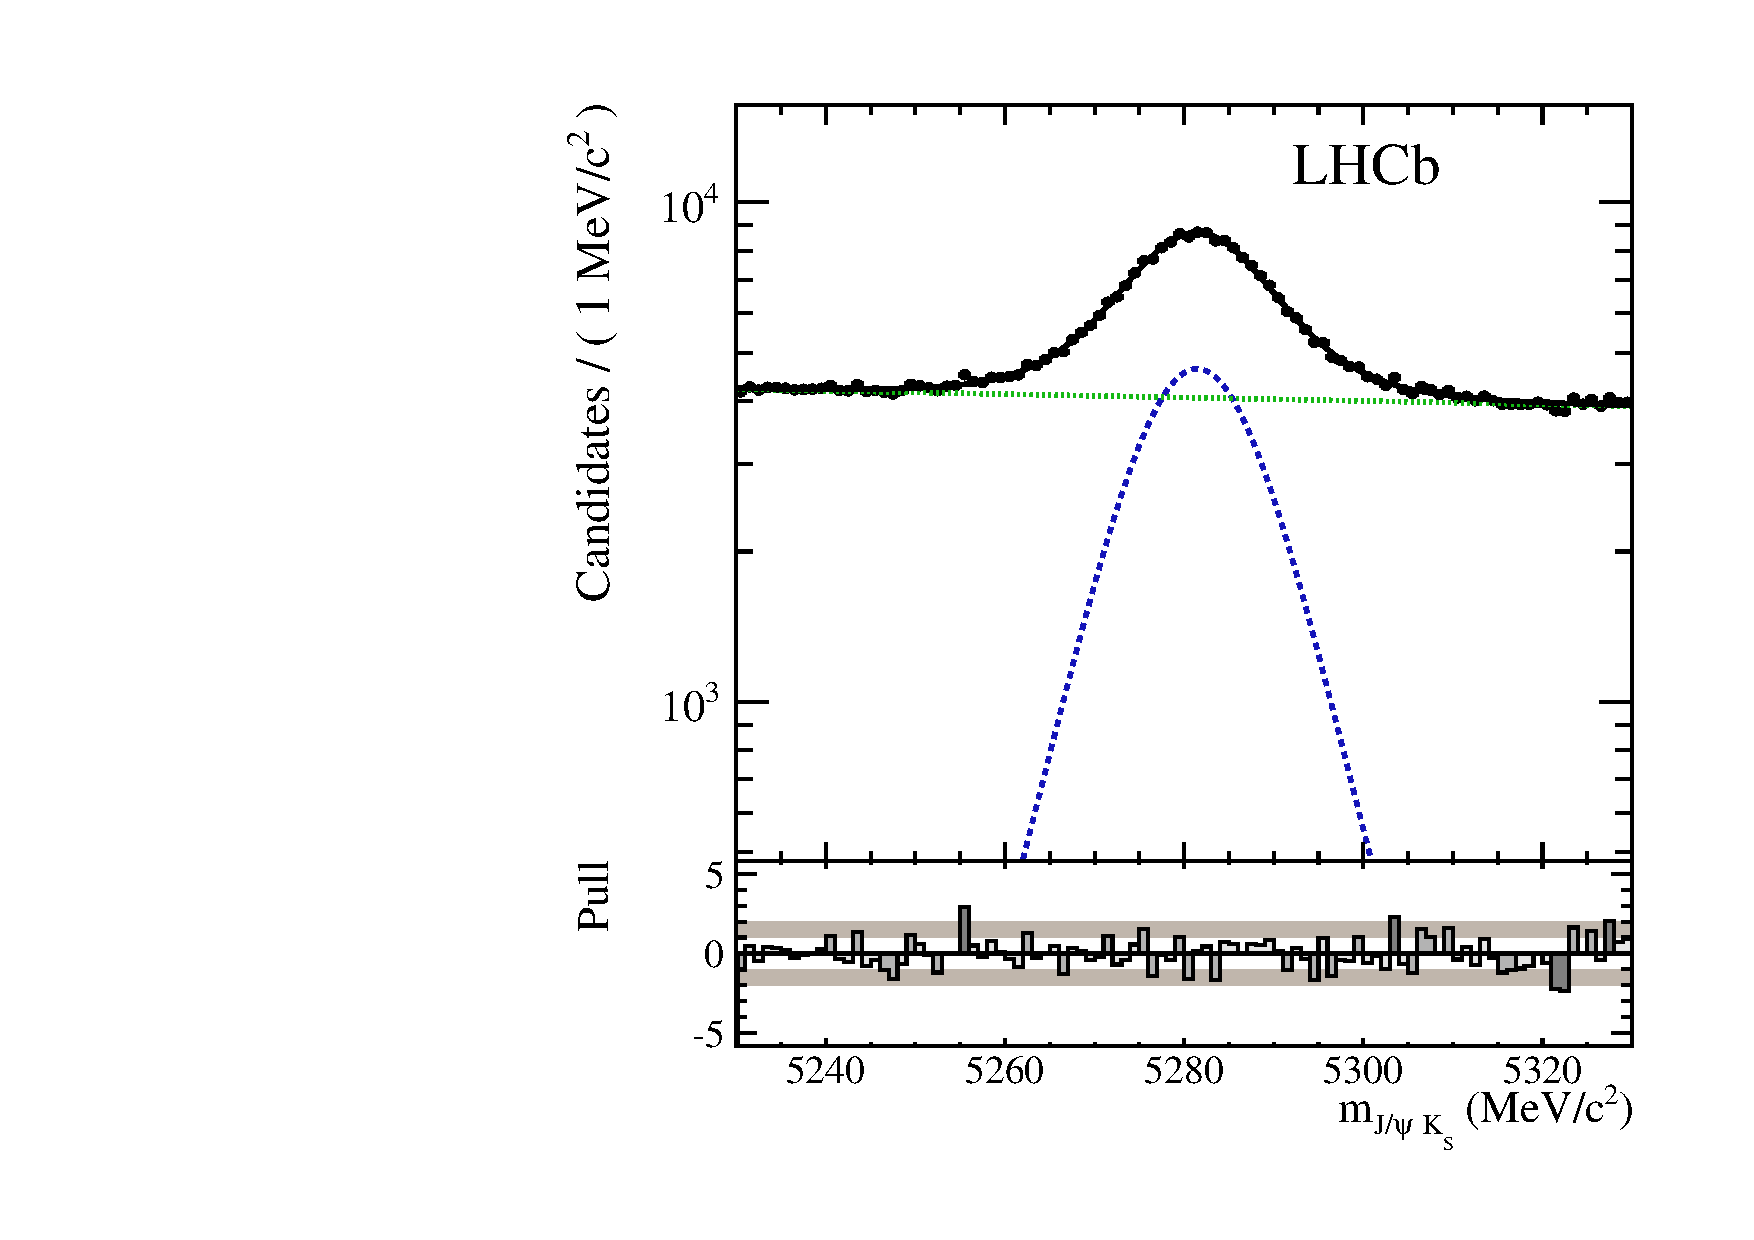
\includegraphics[width=0.49\textwidth]{private/content/measurement-of-sin2beta/figs/offline_splot_downstream.pdf}
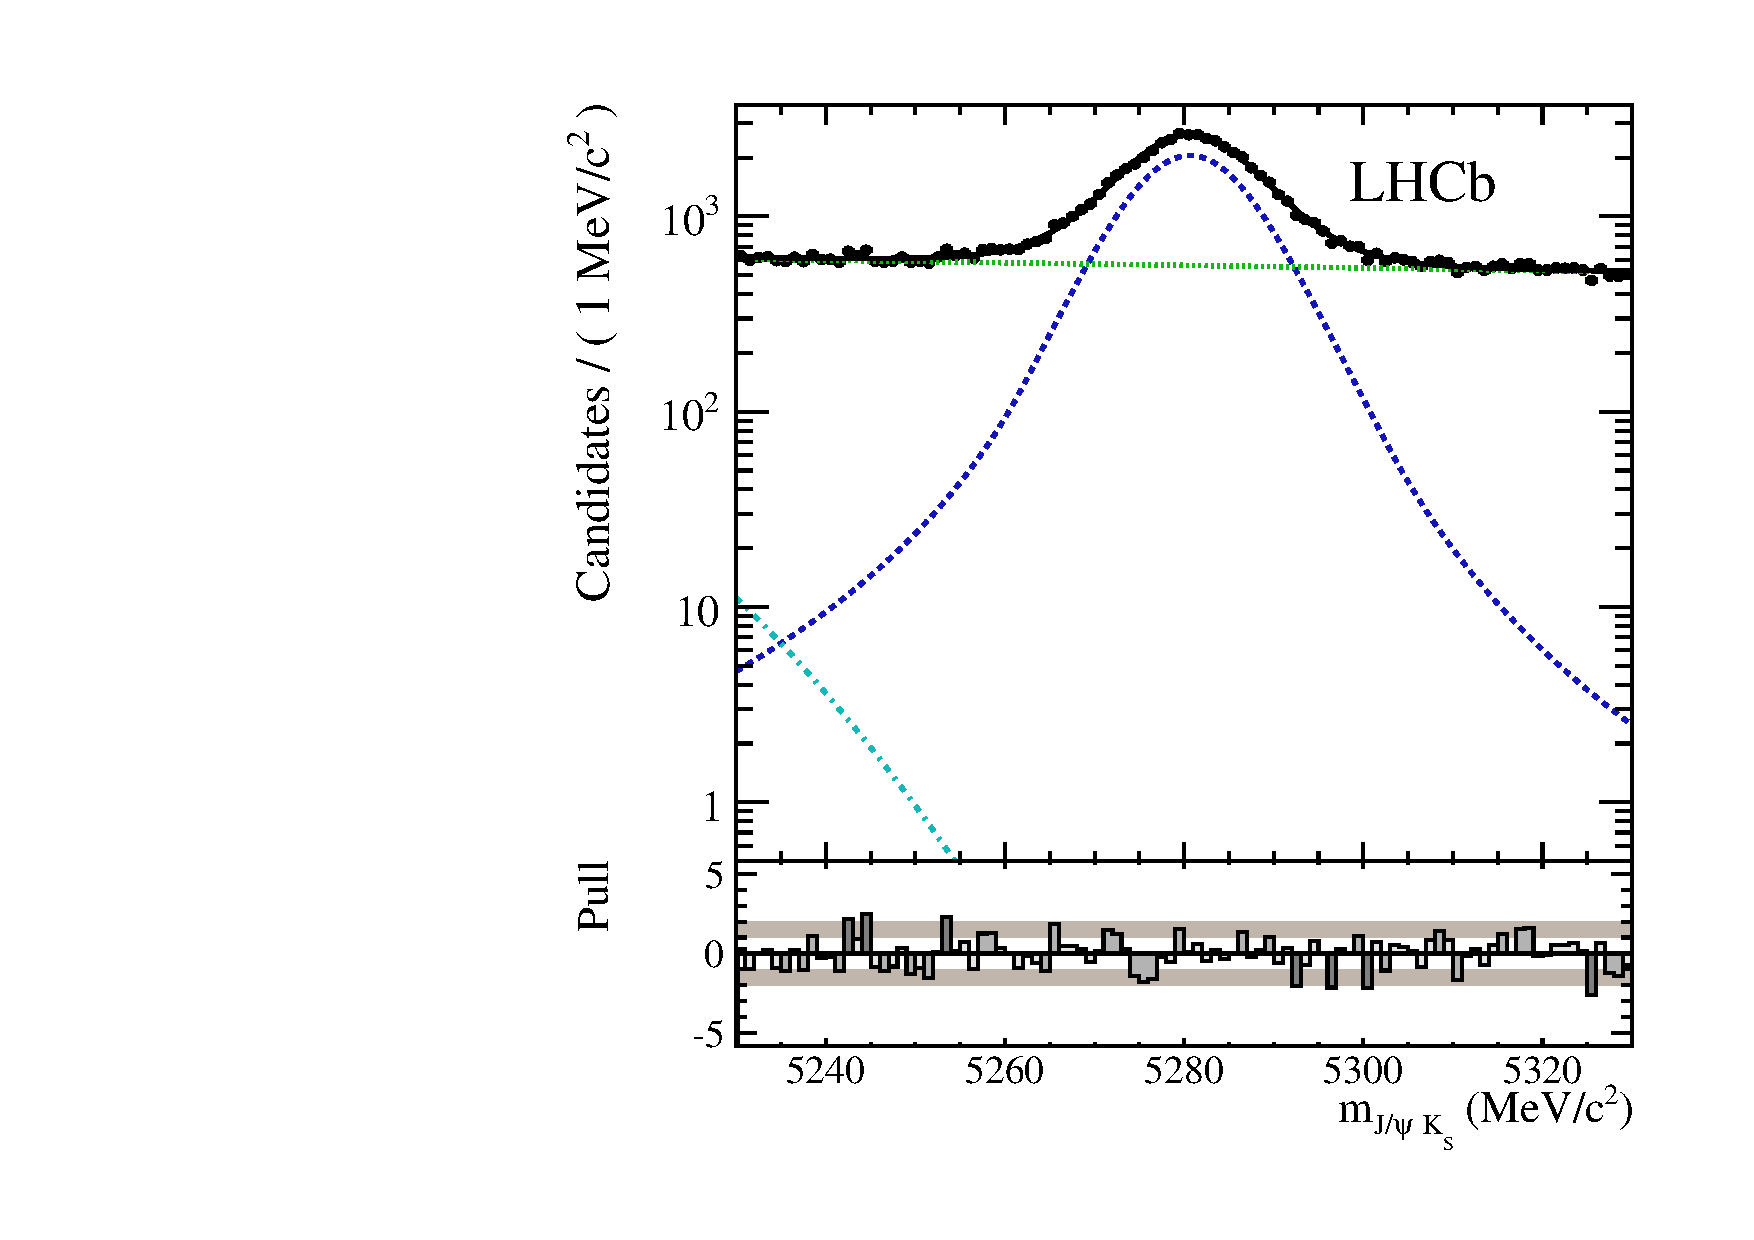
\includegraphics[width=0.49\textwidth]{private/content/measurement-of-sin2beta/figs/offline_splot_longtrack.pdf}
\label{fig:measurement_of_sin2beta:data_preparation:offline_selection:before}
\caption{Mass distribution of the combined 2011 and 2012 data set after
stripping (in logarithmic scale). Only the \PV with the smallest \IP \chisqndf
\wrt the $\Bd$ track is included and--- in case of multiple $\Bd$ candidates---a
random $\Bd$ candidate is chosen. The left plot shows the \catDD, the right one
the \catLL candidates. The solid black line is the projection of the fit \PDF,
the blue dashed line shows the signal, and the green dashed line shows the
background component. For the description of the \catLL candidates, the
additional $\BdToJpsiKstar$ component is depicted as dash-dotted turquoise line.
Below the mass distribution the pull distribution shows the difference of the
bin content and the \PDF value at the bin centre normalized by the error
estimate on the bin content.}
\end{figure}

%...............................................................................
\subsubsection{Sanity cuts}
\label{sec:measurement_of_sin2beta:data_preparation:offline_selection:sanity}

A set of sanity cuts (see
\cref{tab:measurement_of_sin2beta:data_preparation:offline_selection:sanity}) is
applied to remove outliers and ensure that all \DTF fits are converged. The
overall performance shows a signal efficiency of $\SI{99.29}{\percent}$
($\SI{99.75}{\percent}$) and a background rejection of $\SI{6.18}{\percent}$
($\SI{0.75}{\percent}$) in the \catDD (\catLL) sample.
%
\begin{table}
\centering
\caption{Offline selection sanity cuts.}
\label{tab:measurement_of_sin2beta:data_preparation:offline_selection:sanity}
\begin{tabular}{ll}
\toprule
\dtf $\sigma_m$                              & $<\SI[per-mode=symbol]{30}{\MeVcc}$\\
\dtfpv $\obsTimeError$                       & $<\SI[per-mode=symbol]{0.2}{\pico\second}$\\
$\vert z_{\acs*{PV}}\vert$                   & $<\SI{250}{\milli\meter}$\\
\Bd   $\chi_{\text{vtx}}^2/\ndf$             & $<10$\\
\jpsi $\chi_{\text{vtx}}^2/\ndf$             & $<16$\\
\KS   $\chi_{\text{vtx}}^2/\ndf$             & $<20$\\
\dtfpv $\mu$ $p_T$                           & $>\SI[per-mode=symbol]{500}{\MeVc}$\\
$\mu$ $\chi_{\text{track}}^2/\ndf$           & $<3$\\
$\mu$ \acs*{PID}                             & $>0$\\
\dtfpv $\pi\ p$                              & $>\SI[per-mode=symbol]{2000}{\MeVc}$\\
maximal $\pi$ $\chi_{\text{track}}^2/\ndf$   & $<3$\\
minimal $\pi$ \acs*{IP} $\chi^2/\ndf$        & $>4$\\
\multicolumn{2}{c}{\dtf fit and \dtfpv fit converged} \\
\bottomrule
\end{tabular}
\end{table}

%...............................................................................
\subsubsection{Ghost track probability cuts}
\label{sec:measurement_of_sin2beta:data_preparation:offline_selection:ghosts}

To reduce the amount of ghost tracks, a cut on the ghost track probability is
applied, as shown in
\cref{tab:measurement_of_sin2beta:data_preparation:offline_selection:ghosts}.
The overall signal efficiency yields $\SI{95.72}{\percent}$
($\SI{98.09}{\percent}$) with a background rejection of $\SI{26.38}{\percent}$
($\SI{23.36}{\percent}$) for the \catDD (\catLL) sample.
%
\begin{table}
\centering
\caption{Offline selection cuts on ghost track probabilities.}
\label{tab:measurement_of_sin2beta:data_preparation:offline_selection:ghosts}
\begin{tabular}{lll}
\toprule
& \catDD & \catLL\\
\midrule
$\mu$ ghost track probability & \multicolumn{2}{c}{$<0.2$}\\
$\pi$ ghost track probability & \multicolumn{2}{c}{$<0.3$}\\
\bottomrule
\end{tabular}
\end{table}

%...............................................................................
\subsubsection{Cuts on daughter masses and \Lambda mass veto}
\label{sec:measurement_of_sin2beta:data_preparation:offline_selection:daughters}

In order to reduce background contributions due to particle mis-ID (see
\cref{sec:measurement_of_sin2beta:physic_backgrounds}), cuts on the invariant
daughter masses are used as given in
\cref{tab:measurement_of_sin2beta:data_preparation:offline_selection:daughters}.
As long track candidates show a better mass resolution, different cuts are
applied depending on the candidates' track type. These cuts yield a signal
efficiency of $\SI{98.70}{\percent}$ ($\SI{98.92}{\percent}$) and a background
rejection of $\SI{27.53}{\percent}$ ($\SI{39.78}{\percent}$) in the \catDD
(\catLL) sample. The cuts correspond to roughly $8\sigma$ ($4\sigma$) for \catDD
(\catLL) $\KS$ candidates and around $5\sigma$ for the $\jpsi$ candidates.

To reduce pion-proton mis-ID all pion candidate pairs are combined, assigning
the proton mass hypothesis to either one of the pions and recalculating their
invariant mass. An additional requirement on the \proton-\pion \PID of
$\DLLppi<7$ ($<10$) is then applied to all candidates lying inside a
$\pm\SI{7}{\MeVcc}$ ($\pm\SI{5}{\MeVcc}$) region around the \Lambda mass
$M_\Lambda^{\acs*{PDG}} = \SI[per-mode=symbol]{1115.683}{\MeVcc}$ in the \catDD
(\catLL) sample. This \Lambda veto has a signal efficiency of
$\SI{99.32}{\percent}$ ($\SI{99.9}{\percent}$) and a background rejection of
$\SI{10.50}{\percent}$ ($\SI{2.53}{\percent}$) in the \catDD (\catLL) sample.
The cut efficiency on
\LbToJpsiLambda signal \MC is given in
\cref{sec:measurement_of_sin2beta:physic_backgrounds}.
%
\begin{table}
\centering
\caption{Offline selection cuts on the \jpsi and \KS candidates' invariant mass.
($M_{\jpsi}^{\text{\acs*{PDG}}}=\SI{3096.916}{\MeVcc}$,
$M_{\KS}^{\text{\acs*{PDG}}}=\SI{497.614}{\MeVcc}$)}
\label{tab:measurement_of_sin2beta:data_preparation:offline_selection:daughters}
\begin{tabular}{lll}
\toprule
& \multicolumn{1}{c}{\catDD} & \multicolumn{1}{c}{\catLL}\\
\midrule
$m_{\pi\pi}$ & $M_{\KS}^{\text{\acs*{PDG}}}\pm\SI[per-mode=symbol]{55}{\MeVcc}$ & $M_{\KS}^{\text{\acs*{PDG}}}\pm\SI[per-mode=symbol]{15}{\MeVcc}$\\
$m_{\mu\mu}$ & \multicolumn{2}{c}{$M_{\jpsi}^{\text{\acs*{PDG}}}\pm\SI[per-mode=symbol]{60}{\MeVcc}$}\\
\bottomrule
\end{tabular}
\end{table}

%...............................................................................
\subsubsection{DTF fit performance and \KS decay time significance cuts} 
\label{sec:measurement_of_sin2beta:data_preparation:offline_selection:dtf_and_dts}

Finally, cuts on the \dtf fit $\chisqndf<30$ and on the \KS decay time
significance (\wrt to the $\Bd$ decay vertex) of $t_{\KS}/\sigma_{t_{\KS}}>4$
from a \dtfpv fit are applied. These two cuts yield a signal efficiency of
$\SI{99.25}{\percent}$ ($\SI{97.61}{\percent}$) and a background rejection of
$\SI{33.68}{\percent}$ ($\SI{24.89}{\percent}$) for the \catDD (\catLL)
sample.

The fit range is limited to events within $\SI[per-mode=symbol]{0.3}{\pico\second}
<t<\SI[per-mode=symbol]{18.3}{\pico\second}$. Low decay time candidates are
neglected to suppress decay time acceptance effects and prompt background. The
number of candidates with decay times above the limit is negligible. This cut
yields a signal efficiency of $\SI{95.30}{\percent}$ ($\SI{94.86}{\percent}$)
and a background rejection of $\SI{12.77}{\percent}$ ($\SI{25.71}{\percent}$)
for the \catDD (\catLL) sample.

%...............................................................................
\subsubsection{Overall offline selection performance}
\label{sec:measurement_of_sin2beta:data_preparation:offline_selection:total}

\Cref{tab:measurement_of_sin2beta:data_preparation:offline_selection:total}
quotes the overall offline selection performance.
%
\begin{table}
\centering
\caption{Overall offline selection performance.}
\label{tab:measurement_of_sin2beta:data_preparation:offline_selection:total}
\begin{tabular}{lllll}
\toprule
& $\SigEff$ & $\BkgRej$ \\
\midrule
\catDD & $\SI{89.55}{\percent}$ & $\SI{67.61}{\percent}$\\
\catLL & $\SI{89.79}{\percent}$ & $\SI{70.60}{\percent}$\\
\bottomrule
\end{tabular}
\end{table}

% ------------------------------------------------------------------------------
\subsection{Multiple candidates}
\label{sec:measurement_of_sin2beta:data_preparation:multiple_candidates}

As in a typical \LHCb bunch crossing around $\num{2.5}$ visible
\acl{protonproton} collisions occur, the chances are high to find more than one
\PV per recorded event. Choosing the \PV with the smallest \DTF track \IP
\chisqndf \wrt the \Bd candidate is called \emph{best PV selection} in contrast
to a \emph{random PV selection}. Given the small \BdToJpsiKS branching ratio not
more than one signal event can be expected per event. Still, it is possible
that more than one candidate gets reconstructed. From those candidates either
one can be chosen by his \DTF track \IP \chisqndf (\emph{best \Bd candidate
selection}) or as well randomly (\emph{random \Bd candidate selection}). Instead
of consecutively selecting a \PV and \Bmeson candidate a joint decision can be
made. Each $(\text{\acs{PV}}, \Bd)$ pair can again be chosen either based on
the best fit quality or by random.

After stripping selection around $\SI{2}{\percent}$ of the events contain more
than one \Bd candidate and $\SIrange[range-phrase = -, range-units = single]
{4}{5}{\percent}$ of all \Bmeson candidates are not unique in their event 
(\cf \cref{tab:measurement_of_sin2beta:data_preparation:multiple_candidates:after_stripping}).
%
\begin{table}
\centering
\caption{
Number of multiple \BdToJpsiKS candidates after stripping. The numbers in the
first row represent the fraction of \Bd candidates that are not \emph{unique} in
an event, \ie the event contains more than one candidate. The numbers in the
second row show the fraction of events with multiple \Bd candidates.
Additionally, a listing of the occurrence of events with different numbers of
multiple \Bd candidates is given. The last row shows the fraction of \Bd
candidates that need to be discarded in order to only get events with a single
\Bd candidate.}
\label{tab:measurement_of_sin2beta:data_preparation:multiple_candidates:after_stripping}
\begin{tabular}{lcccc}
\toprule
 & \multicolumn{2}{c}{2011} & \multicolumn{2}{c}{2012}\\
\midrule
fraction of multiple & \multicolumn{2}{c}{\multirow{2}[2]{*}{\SI{4.2}{\percent}}} & \multicolumn{2}{c}{\multirow{2}[2]{*}{\SI{4.9}{\percent}}}\\
\Bd candidates & & & & \\
\midrule
fraction of events with & \multicolumn{2}{c}{\multirow{2}[2]{*}{\SI{2.1}{\percent}}} & \multicolumn{2}{c}{\multirow{2}[2]{*}{\SI{2.4}{\percent}}}\\
 multiple \Bd candidates & & & & \\  
\cmidrule(r){2-5}
 & \#\Bd cands & \#events & \#\Bd cands & \#events\\
\cmidrule(r){2-5}
 & 1 & 575780 & 1 & 1482895\\
 & 2 & 11997  & 2 & 35921\\
 & 3 & 382    & 3 & 1223\\
 & 4 & 50     & 4 & 194\\
 & 5 & 4      & 5 & 9\\
 & 6 & 1      & 6 & 9\\
 & 7 & 0      & 7 & 1\\
\midrule
fraction of \Bd candidates & \multicolumn{2}{c}{\multirow{2}[2]{*}{\SI{2.2}{\percent}}} & \multicolumn{2}{c}{\multirow{2}[2]{*}{\SI{2.5}{\percent}}}\\
to discard & & & & \\
\bottomrule
\end{tabular}
\end{table}
%
After stripping and subsequent offline selection roughly $\SI{0.3}{\percent}$ of
events contain multiple \Bd candidates while in $\SI{6}{\percent}$ of the events
more than one \PV is found. 
\Cref{tab:measurement_of_sin2beta:data_preparation:multiple_candidates:after_selection} 
presents the detailed numbers for multiple \PV and \Bd candidates after
stripping and offline selection. Of the remaining (\acs{PV},\Bd) pairs one is
chosen randomly
%
\begin{table}
\centering
\caption{ 
Number of multiple candidates after stripping and selection. The numbers in the
first row represent the fraction of (\PV,\Bd) candidate pairs that are not
unique in an event. The numbers in the second row show the fraction of events
with multiple (\PV,\Bd) candidate pairs.  The third row includes the numbers of
event with multiple \Bd candidates. Additionally, a listing of the occurrence of
events with different numbers of multiple \Bd candidates is given. After that,
the number of \Bd candidates to discard is given. In the fourth row the number
of events containing multiple \acp{PV} is listed together with the detailed
description of the frequency of multiple \acp{PV} per event. The last row shows
the fraction of (\PV,\Bd) candidate pairs that need to be discarded in order to
only keep one (\PV,\Bd) candidate per event. }
\label{tab:measurement_of_sin2beta:data_preparation:multiple_candidates:after_selection}
\begin{tabular}{lcccc}
\toprule
 & \multicolumn{2}{c}{2011} & \multicolumn{2}{c}{2012}\\
\midrule
fraction of multiple & \multicolumn{2}{c}{\multirow{2}[2]{*}{\SI{12.5}{\percent}}} & \multicolumn{2}{c}{\multirow{2}[2]{*}{\SI{12.8}{\percent}}}\\
candidates & & & & \\
\midrule
fraction of events with& \multicolumn{2}{c}{\multirow{2}[2]{*}{\SI{6.0}{\percent}}} & \multicolumn{2}{c}{\multirow{2}[2]{*}{\SI{6.1}{\percent}}}\\
multiple (\acs{PV},\Bd) candidates & & & & \\  
\midrule
fraction of events with & \multicolumn{2}{c}{\multirow{2}[2]{*}{\SI{0.3}{\percent}}} & \multicolumn{2}{c}{\multirow{2}[2]{*}{\SI{0.4}{\percent}}}\\
multiple \Bd candidates & & & & \\  
\cmidrule(r){2-5}
 & \#\Bd cands & \#events & \#\Bd cands & \#events\\
\cmidrule(r){2-5}
 & 1 & 74065 & 1 & 165915\\
 & 2 & 253   & 2 & 635\\
 & 3 & 0     & 3 & 3\\
 \midrule
fraction of \Bd candidates & \multicolumn{2}{c}{\multirow{2}[2]{*}{\SI{0.3}{\percent}}} & \multicolumn{2}{c}{\multirow{2}[2]{*}{\SI{0.4}{\percent}}}\\
to discard & & & & \\
 \midrule
fraction of events & \multicolumn{2}{c}{\multirow{2}[2]{*}{\SI{5.7}{\percent}}} & \multicolumn{2}{c}{\multirow{2}[2]{*}{\SI{5.8}{\percent}}}\\
with multiple \acp{PV} & & & & \\  
\cmidrule(r){2-5}
 & \#\acsp{PV} & \#events & \#\acsp{PV} & \#events\\
\cmidrule(r){2-5}
 & 1 & 69755 & 1 & 156211\\
 & 2 & 4279  & 2 & 9583\\
 & 3 & 265   & 3 & 692\\
 & 4 & 19    & 4 & 58\\
 & 5 & 0     & 5 & 9\\
\midrule
fraction of (\acs{PV},\Bd) candidate & \multicolumn{2}{c}{\multirow{2}[2]{*}{\SI{6.5}{\percent}}} & \multicolumn{2}{c}{\multirow{2}[2]{*}{\SI{6.6}{\percent}}}\\
pairs to discard & & & & \\
\bottomrule
\end{tabular}
\end{table}

% ------------------------------------------------------------------------------
\subsection{\acs{MC} and data samples}
\label{sec:measurement_of_sin2beta:data_preparation:datasamples}

Over the course of the described measurement several datasets are utilised such
as recorded data from the \LHCb experiment as well as simulated data.

All candidates in the nominal dataset finally used for the fit to estimate the
\CP observables \SJpsiKS and \CJpsiKS pass the given trigger configuration, the
detached stripping selection, and the described offline selection leaving
$\num{114000}$ signal candidates. The analysis only makes use of $\num{42000}$
tagged signal candidates.
\Cref{tab:measurement_of_sin2beta:data_preparation:datasamples:numbers} lists
the numbers of tagged signal candidates split into subsamples of tagger,
trigger, track type, and year of data-taking.
%
\begin{table}
\centering
\caption{Number of tagged signal candidates split into categories of tagger, 
trigger, track type, and year of data-taking. All numbers rounded.}
\label{tab:measurement_of_sin2beta:data_preparation:datasamples:numbers}
\begin{tabular}{c|c|c|c|c|c|c|c|c|c|c}
\toprule
\multicolumn{1}{c}{} & \multicolumn{5}{c}{DD} & \multicolumn{5}{c}{LL}\\
\midrule
\multirow{6}[6]{*}{\catOO} & \multirow{2}[2]{*}{\catOS} & \catAU & \num{5134} & \multirow{2}[2]{*}{\num{5991}} & \multirow{6}[6]{*}{\num{9423}} & \multirow{2}[2]{*}{\catOS} & \catAU & \num{2263} & \multirow{2}[2]{*}{\num{2597}} & \multirow{6}[6]{*}{\num{3799}}\\
\cmidrule(r){3-4}\cmidrule(r){8-9}
& & \catEB & \num{857} & & & & \catEB & \num{334} & & \\
\cmidrule(r){2-5}\cmidrule(r){7-10}
 & \multirow{2}[2]{*}{\catSS} & \catAU & \num{2028} & \multirow{2}[2]{*}{\num{2352}} & & \multirow{2}[2]{*}{\catSS} & \catAU & \num{744} & \multirow{2}[2]{*}{\num{834}} & \\
 \cmidrule(r){3-4}\cmidrule(r){8-9}
 & & \catEB & \num{324} & & & & \catEB & \num{90} & & \\
\cmidrule(r){2-5}\cmidrule(r){7-10}
 & \multirow{2}[2]{*}{BS} & \catAU & \num{941} & \multirow{2}[2]{*}{\num{1080}} & & \multirow{2}[2]{*}{BS} & \catAU & \num{321} & \multirow{2}[2]{*}{\num{368}} & \\
 \cmidrule(r){3-4}\cmidrule(r){8-9}
 & & \catEB & \num{139} & & & & \catEB & \num{47} & & \\
 \midrule
\multirow{6}[6]{*}{\catOT} & \multirow{2}[2]{*}{\catOS} & \catAU & \num{10378} & \multirow{2}[2]{*}{\num{12567}} & \multirow{6}[6]{*}{\num{20160}} & \multirow{2}[2]{*}{\catOS} & \catAU & \num{4599} & \multirow{2}[2]{*}{\num{5571}} & \multirow{6}[6]{*}{\num{8178}}\\
\cmidrule(r){3-4}\cmidrule(r){8-9}
& & \catEB & \num{2189} & & & & \catEB & \num{972} & & \\
\cmidrule(r){2-5}\cmidrule(r){7-10}
 & \multirow{2}[2]{*}{\catSS} & \catAU & \num{4247} & \multirow{2}[2]{*}{\num{5226}} & & \multirow{2}[2]{*}{\catSS} & \catAU & \num{1550} & \multirow{2}[2]{*}{\num{1831}} & \\
 \cmidrule(r){3-4}\cmidrule(r){8-9}
 & & \catEB & \num{979} & & & & \catEB & \num{281} & & \\
\cmidrule(r){2-5}\cmidrule(r){7-10}
 & \multirow{2}[2]{*}{BS} & \catAU & \num{1963} & \multirow{2}[2]{*}{\num{2367}} & & \multirow{2}[2]{*}{BS} & \catAU & \num{658} & \multirow{2}[2]{*}{\num{776}} & \\
 \cmidrule(r){3-4}\cmidrule(r){8-9}
 & & \catEB & \num{404} & & & & \catEB & \num{118} & & \\
\bottomrule
\end{tabular}
\label{tab:data_preparation:nominal}
\end{table}
%
\begin{figure}[!htb]
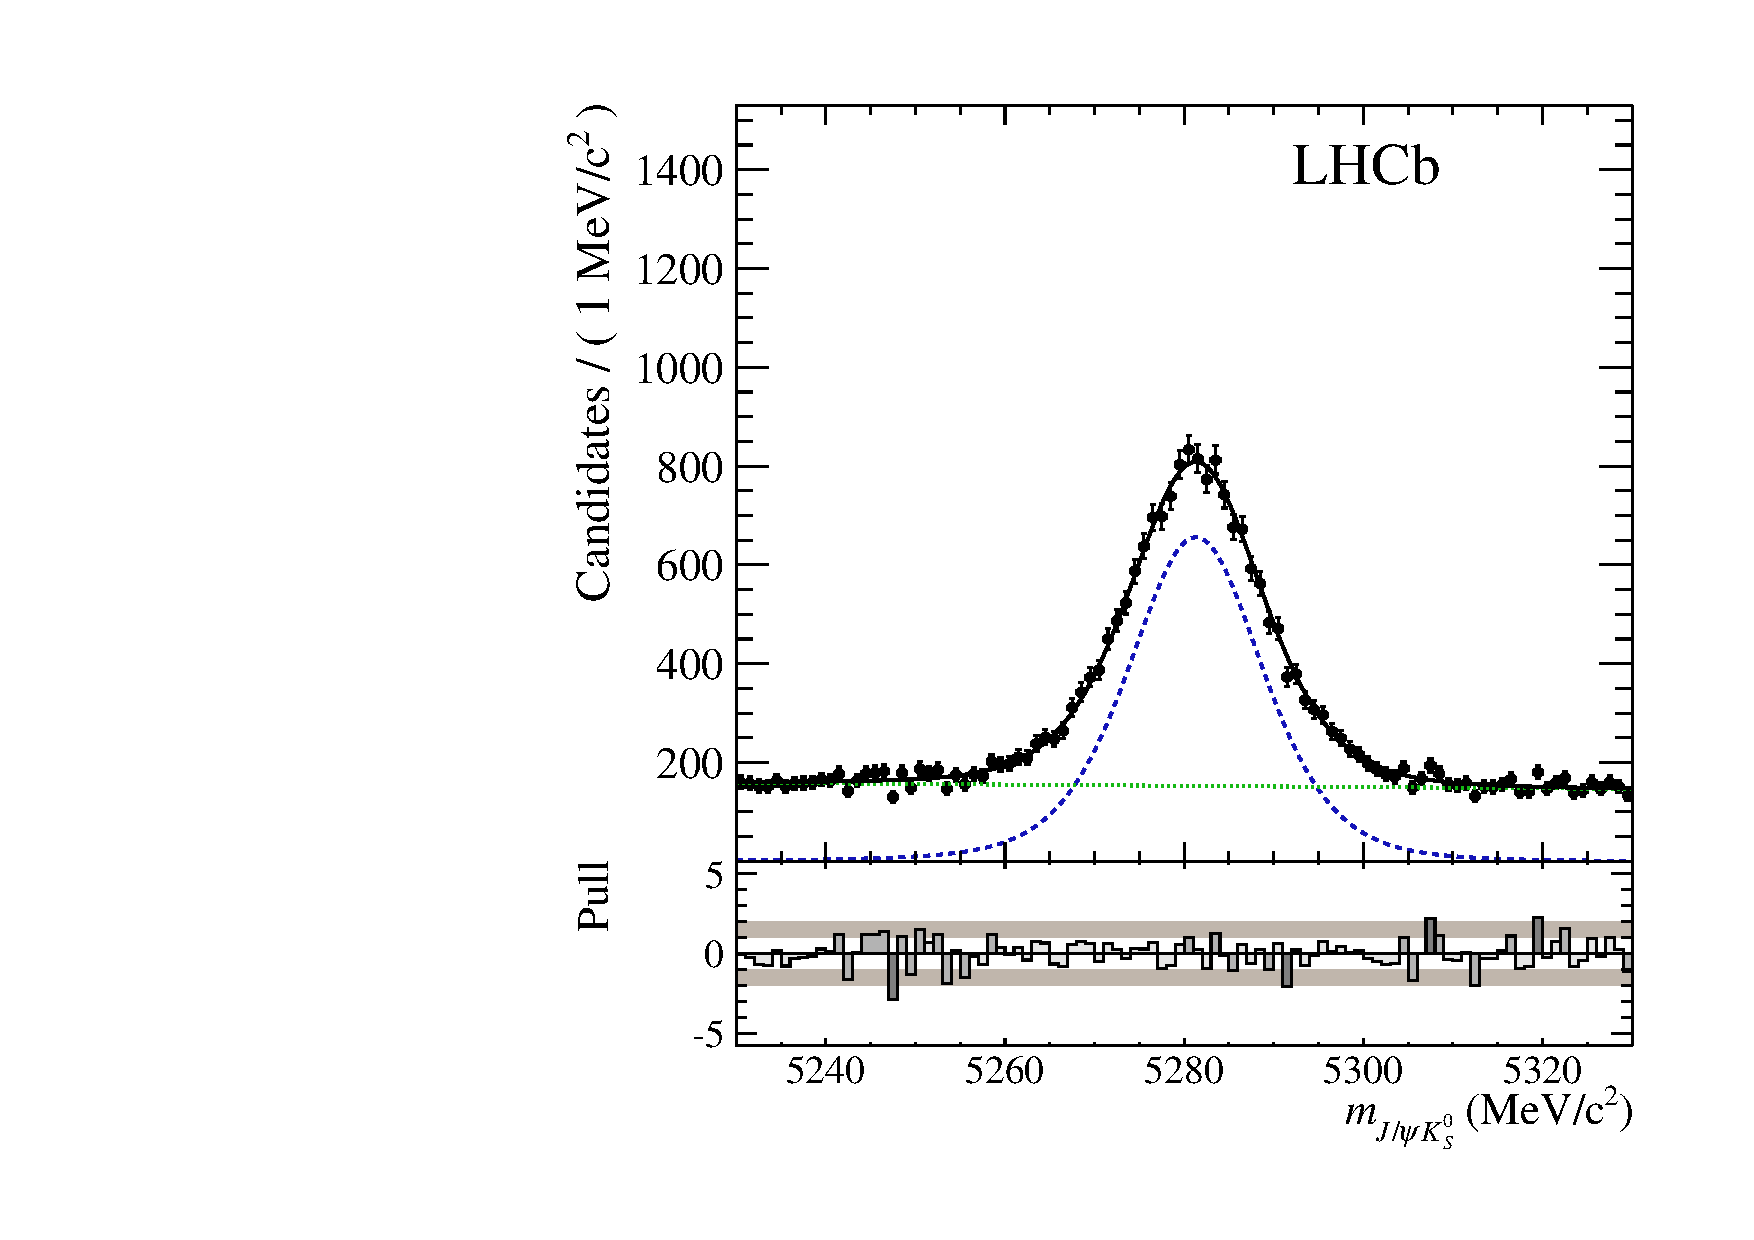
\includegraphics[width=0.49\textwidth]{private/content/measurement-of-sin2beta/figs/mass_11.pdf}
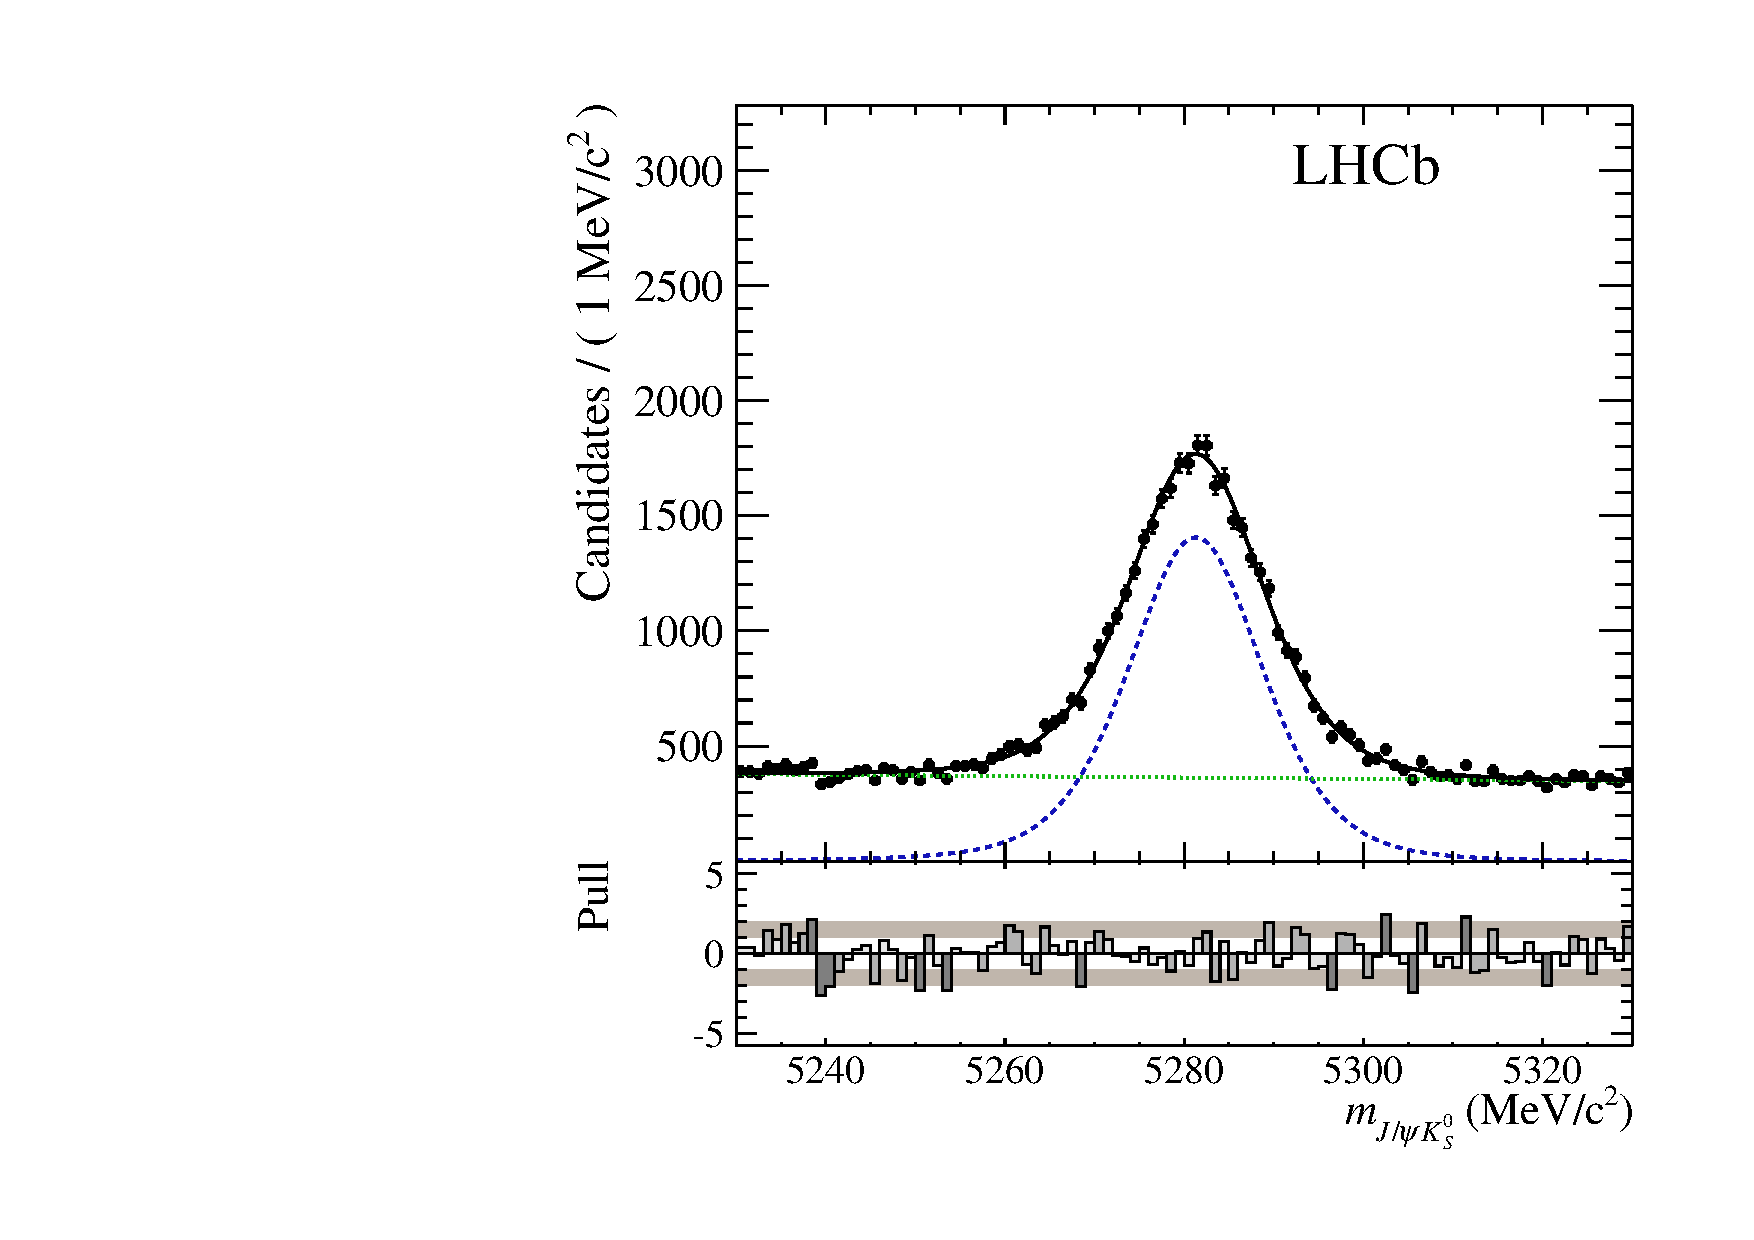
\includegraphics[width=0.49\textwidth]{private/content/measurement-of-sin2beta/figs/mass_12.pdf}
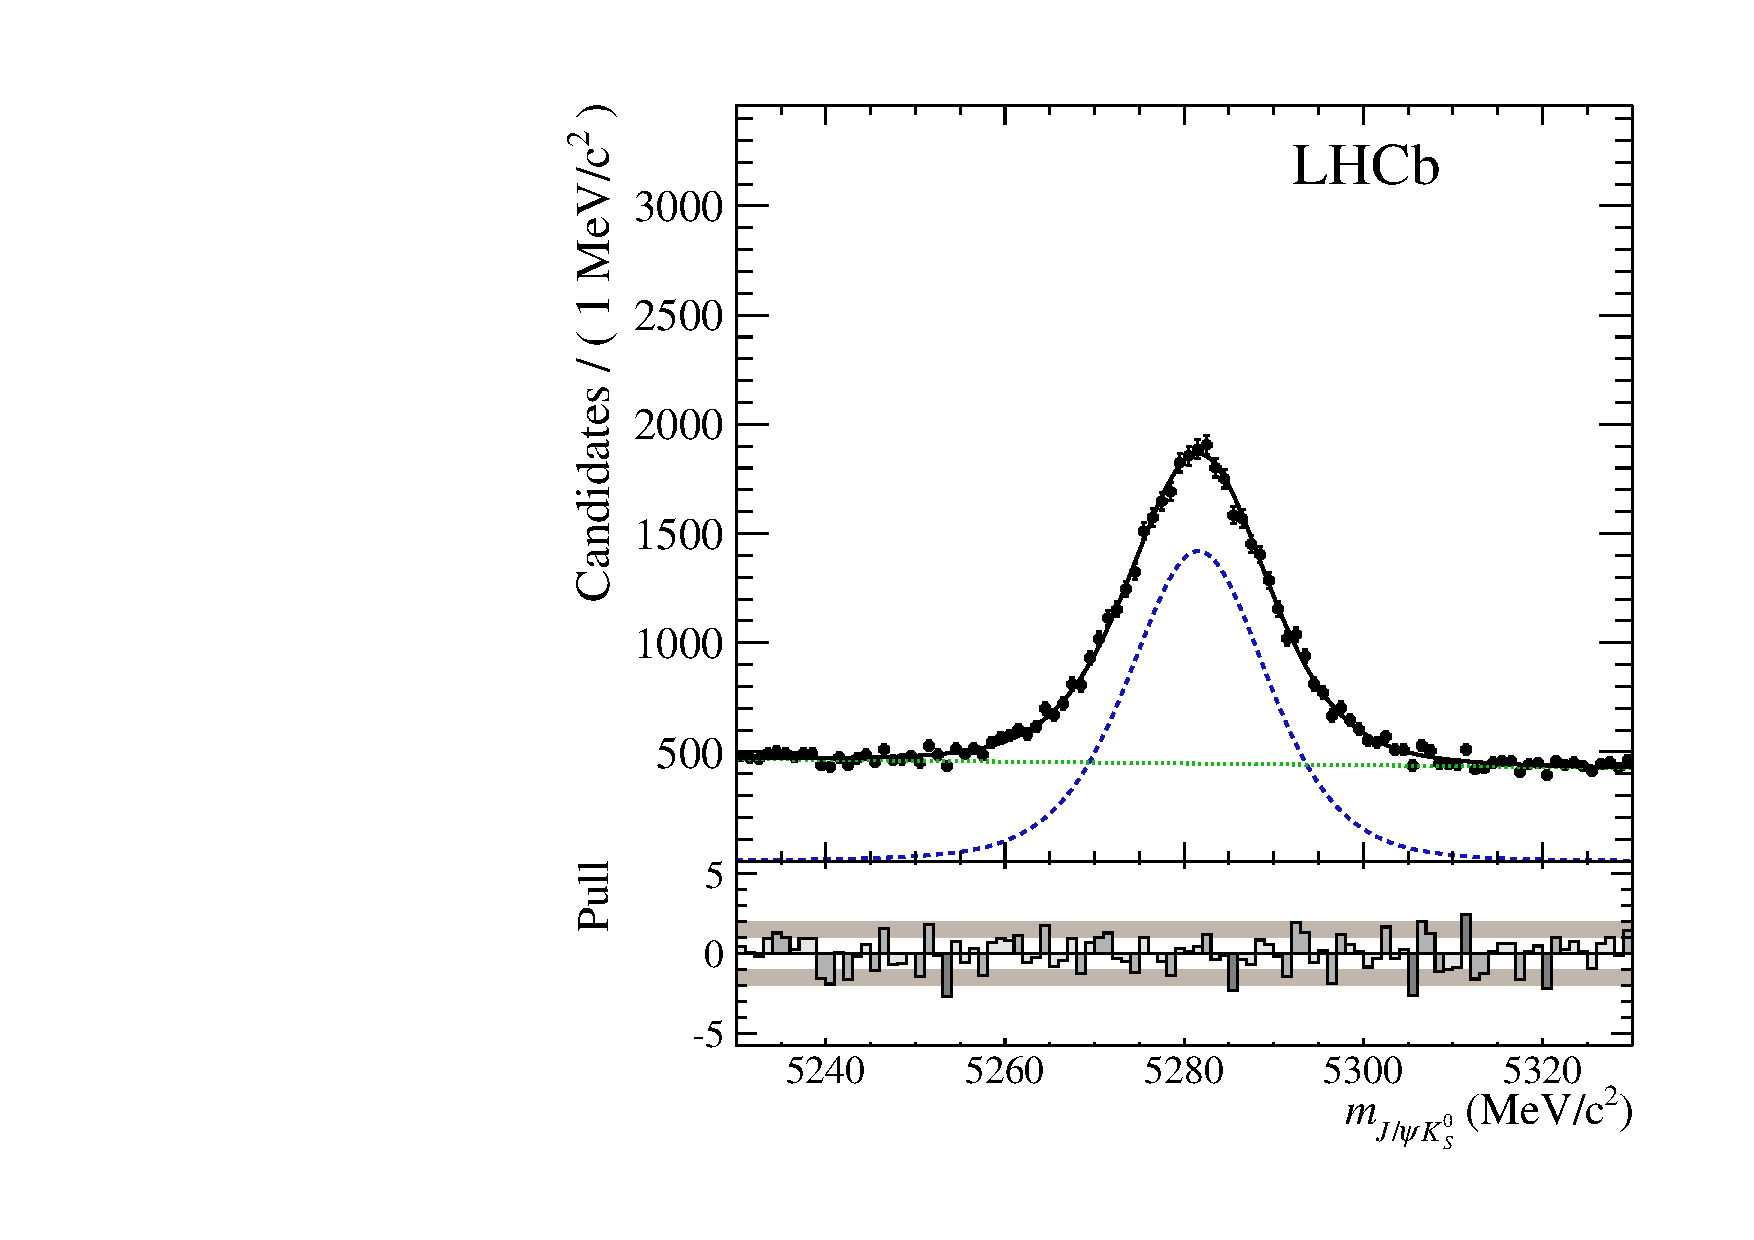
\includegraphics[width=0.49\textwidth]{private/content/measurement-of-sin2beta/figs/mass_DD.pdf}
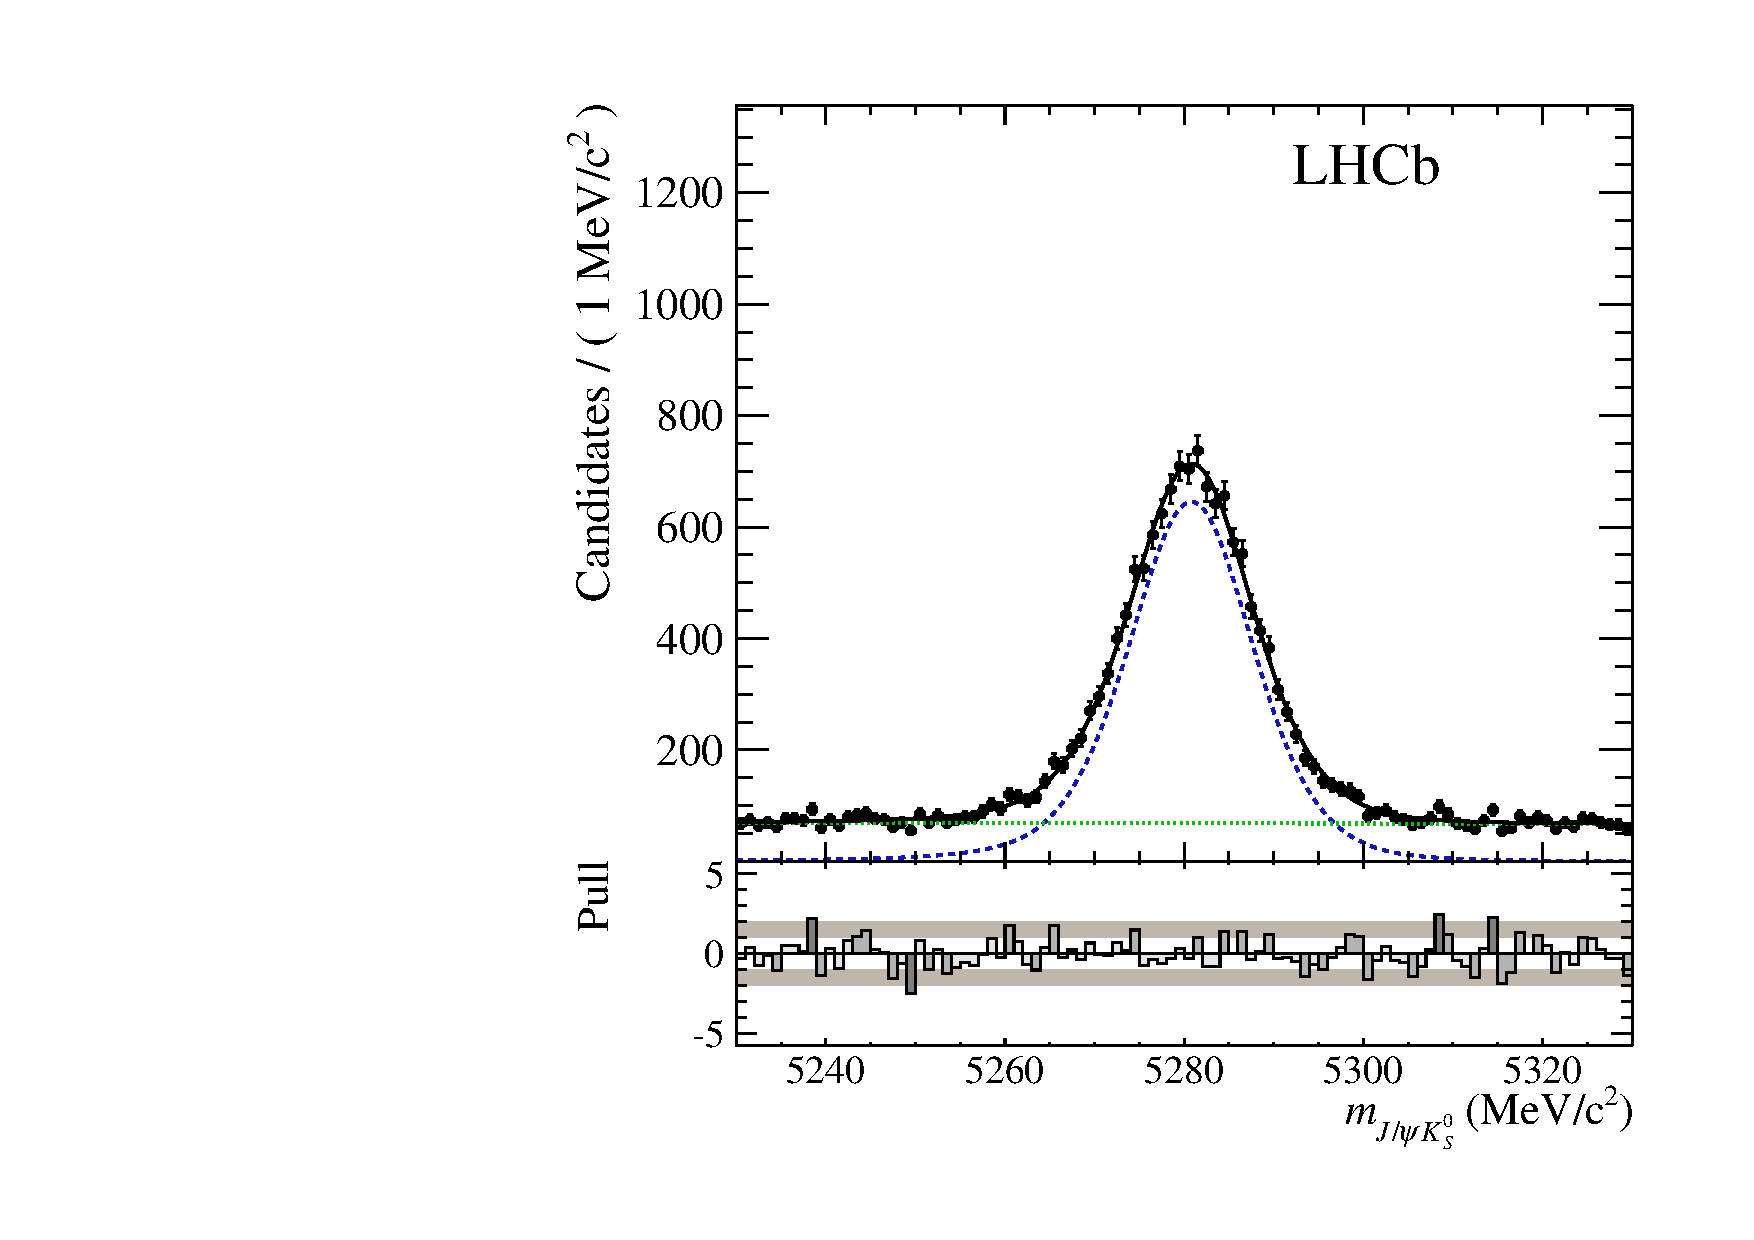
\includegraphics[width=0.49\textwidth]{private/content/measurement-of-sin2beta/figs/mass_LL.pdf}
\label{fig:measurement_of_sin2beta:data_preparation:datasamples:split}
\caption{Mass distribution of the nominal data set, split into year of
data-taking and into $\KS$ track type. Top row: on the left \catOO, on the right
\catOT. Bottom row: on the left \catDD, on the right \catLL. The solid black
line shows the fit projection of the nominal mass \PDF (see
\cref{missing}). The blue dashed line shows the signal, the green dashed line
the background component.}
\end{figure}
%
\begin{figure}
\centering
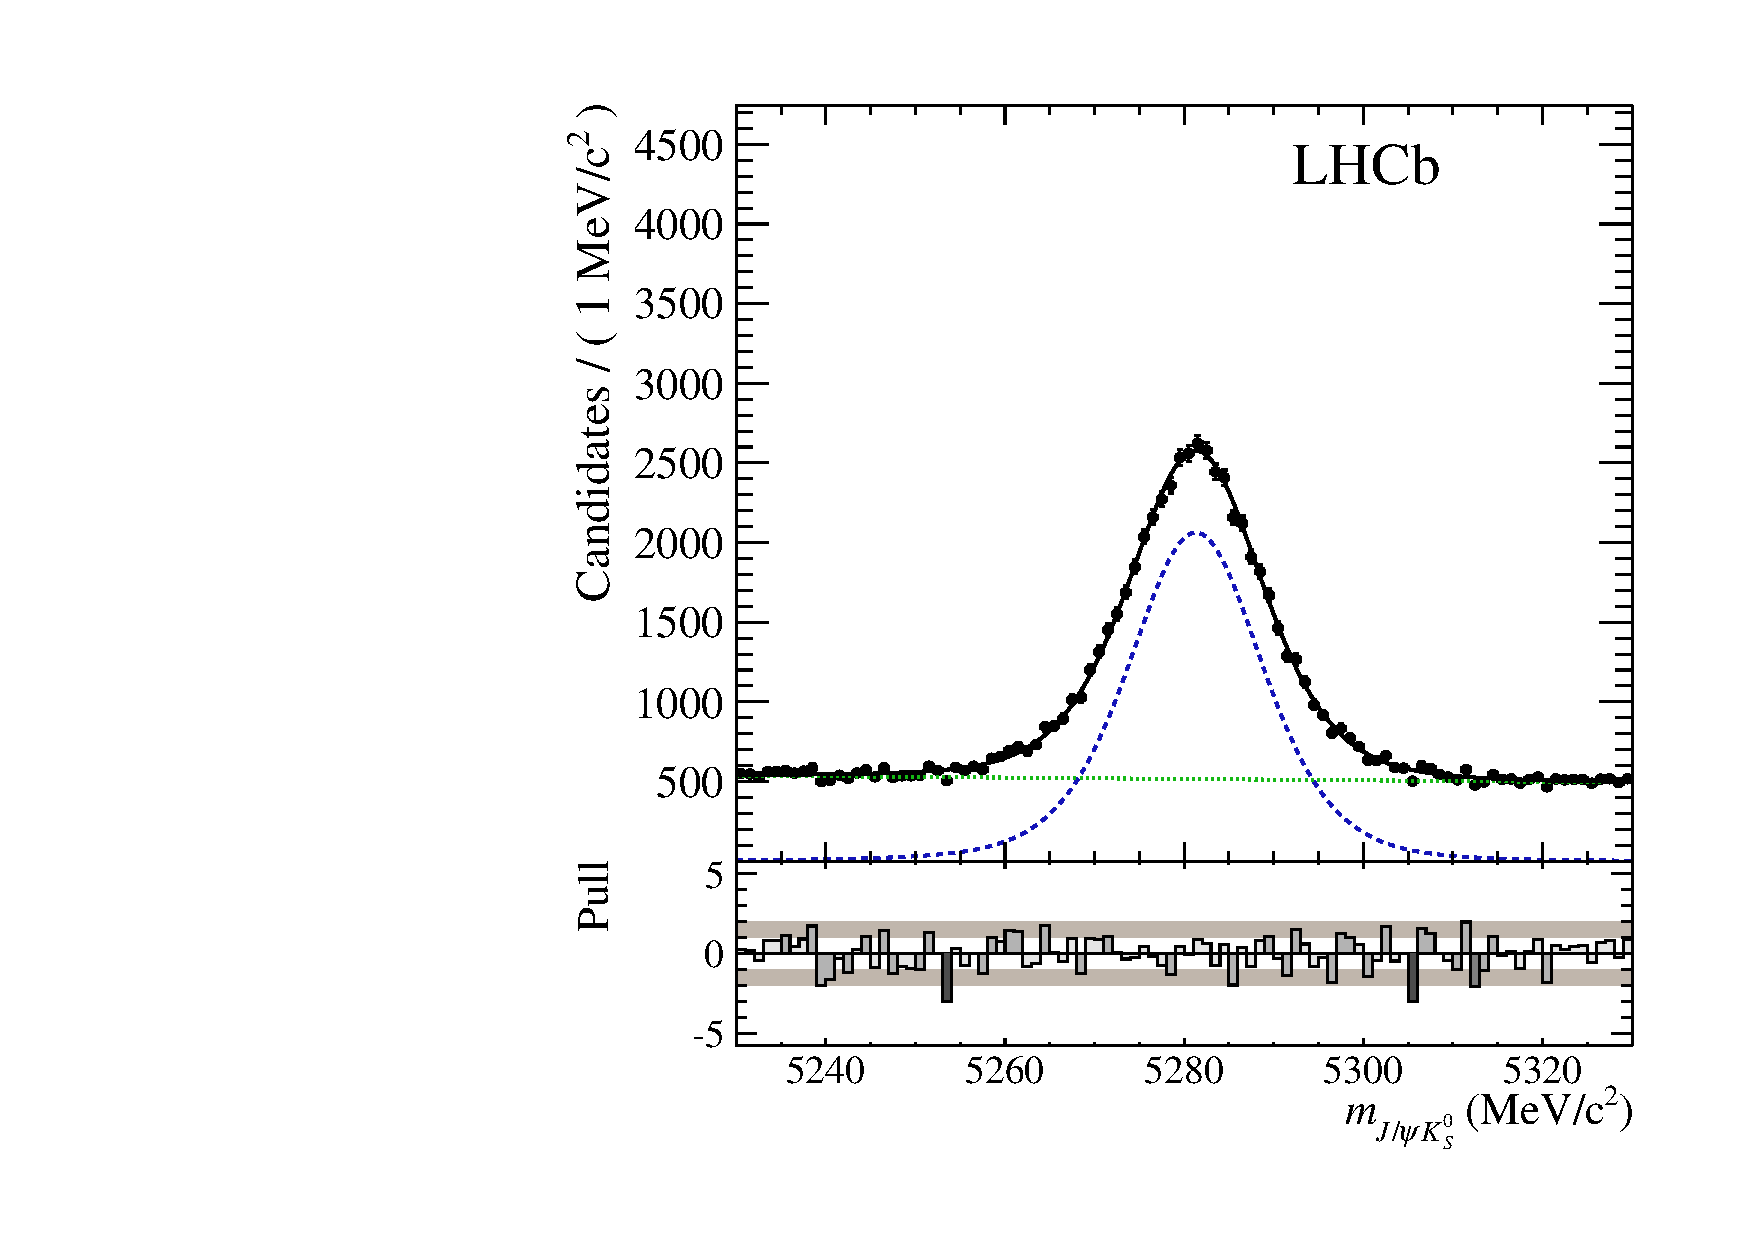
\includegraphics[width=0.8\textwidth]{private/content/measurement-of-sin2beta/figs/mass.pdf}
\label{fig:measurement_of_sin2beta:data_preparation:datasamples:combined}
\caption{Combined mass distribution of the nominal data set for all different
categories. The solid black line shows the fit projection of the nominal mass
\PDF (see section \cref{missing}). The blue dashed line shows the
signal, the green dashed line the background component.}
\end{figure}
\addref{Description of mass PDF}

%...............................................................................
\subsubsection{\MC datasets}
\label{sec:measurement_of_sin2beta:data_preparation:datasamples:mc}

The \acf{MC} samples are produced using \PythiaSix and \PythiaEight in the
generation step. An equal amount of events is generated using each generator
version and also for both possible magnet polarities called \emph{up} and
\emph{down}. Also different samples are produced for \catOO and \catOT running
conditions. Heavy particles from generated \protonproton collisions are decayed
using \EvtGen and the particle interactions with the \LHCb detector material is
handled by \GeantFour. The \EvtGen physics model is set to \Verb=SSD_CP= with
parameters as summarised in
\cref{tab:measurement_of_sin2beta:data_preparation:datasamples:mc:decfile}. The
detector response is simulated using \Boole. The \LHCb trigger software \Moore,
the reconstruction based on \Brunel and the stripping selection using \DaVinci
treat simulated and recorded data in the same manner.
\info{Quote software versions? FT package?}
%
\begin{table}[!htb]
\centering
\caption{Physics parameters used in the simulation.}
\label{tab:measurement_of_sin2beta:data_preparation:datasamples:mc:decfile}
\begin{tabular}{ll}
\toprule
Parameter                            & Generation value \\
\midrule
$\dmd$                               & \SI{0.502e12}{(\planckbar\per\second)} \\
$\frac{\DG}{\Gamma}$                 & \num{0} \\
$\left\vert\frac{q}{p}\right\vert$   & \num{1} \\
$\arg(\frac{q}{p})$                  & \num{-0.775} \\
$\vert A_f \vert$                    & \num{1} \\
$\arg(A_f)$                          & \num{0} \\
$\left\vert A_{\bar{f}} \right\vert$ & \num{-1}  \\
$\arg(A_{\bar{f}})$                  & \num{0} \\
$\tau$                               & \SI{1.519068}{\pico\second}\\
\bottomrule
\end{tabular}
\end{table}
%
Studies to check for possible background contributions from partly reconstructed
decays or decays with mis-identified particles (outlined in
\cref{sec:measurement_of_sin2beta:physic_backgrounds}) require several inclusive
and signal \MC samples using the same conditions as for the nominal \MC data
set. \Cref{tab:measurement_of_sin2beta:data_preparation:datasamples:mc:samples}
shows the used \MC data sets and gives the number of generated events.
%
\begin{table}[!htb]
\centering
\caption{Inclusive and signal MC data sets used in this analysis, with the
generated number of events and if possible an estimate on the corresponding
integrated luminosity.}
\label{tab:measurement_of_sin2beta:data_preparation:datasamples:mc:samples}
\begin{tabular}{lll}
\toprule
\acs{MC} name & \# events & int.\ lumi.\ $[\si{\per\fb}]$ \\ 
\midrule
inclJpsi    & \SI{60}{M} & -             \\
Bd2JpsiX    & \SI{20}{M} & -             \\
Bu2JpsiX    & \SI{20}{M} & -             \\
Bs2JpsiX    & \SI{20}{M} & -             \\
Bd2JpsiKst  & \SI{4}{M}  & $\approx 1.6$ \\
Lb2JpsiL    & \SI{3}{M}  & $\approx 15$  \\
\bottomrule
\end{tabular}
\end{table}
